\newpage
\section{Diffraction substraction}

To account the diffraction produced by the secondary a model in the GRASP software was made using the APEX telescope parameters.
The result was transformed to the surface error and scaled to match a grid of 256x256 pixels that is the common pixel size used in APEX holography pipelines. If a map of different pixel size is used a 2D interpolation is made to match the map size.

The figure \ref{fig:grasp_diffraction} shows the GRASP diffraction model, this model is substracted from the large scale corrected map. The figure \ref{fig:diffraction_corrected} shows the effect of the diffraction model substraction.


\begin{figure}
    \centering
    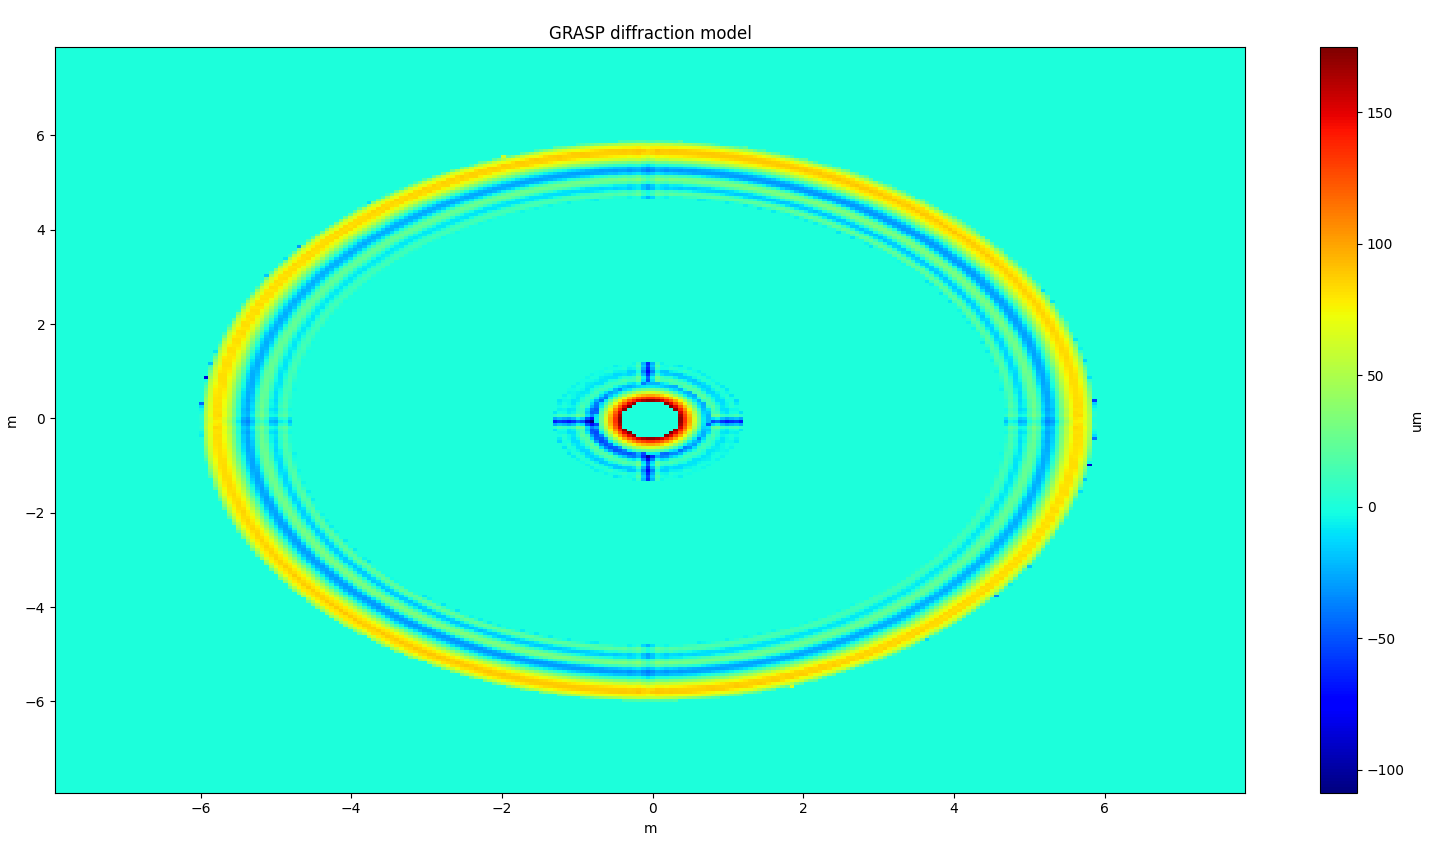
\includegraphics[width=0.8\textwidth]{images/grasp_diffraction_model.png}
    \caption{GRASP diffraction model.}
    \label{fig:grasp_diffraction}
\end{figure}


\begin{figure}
    \centering
    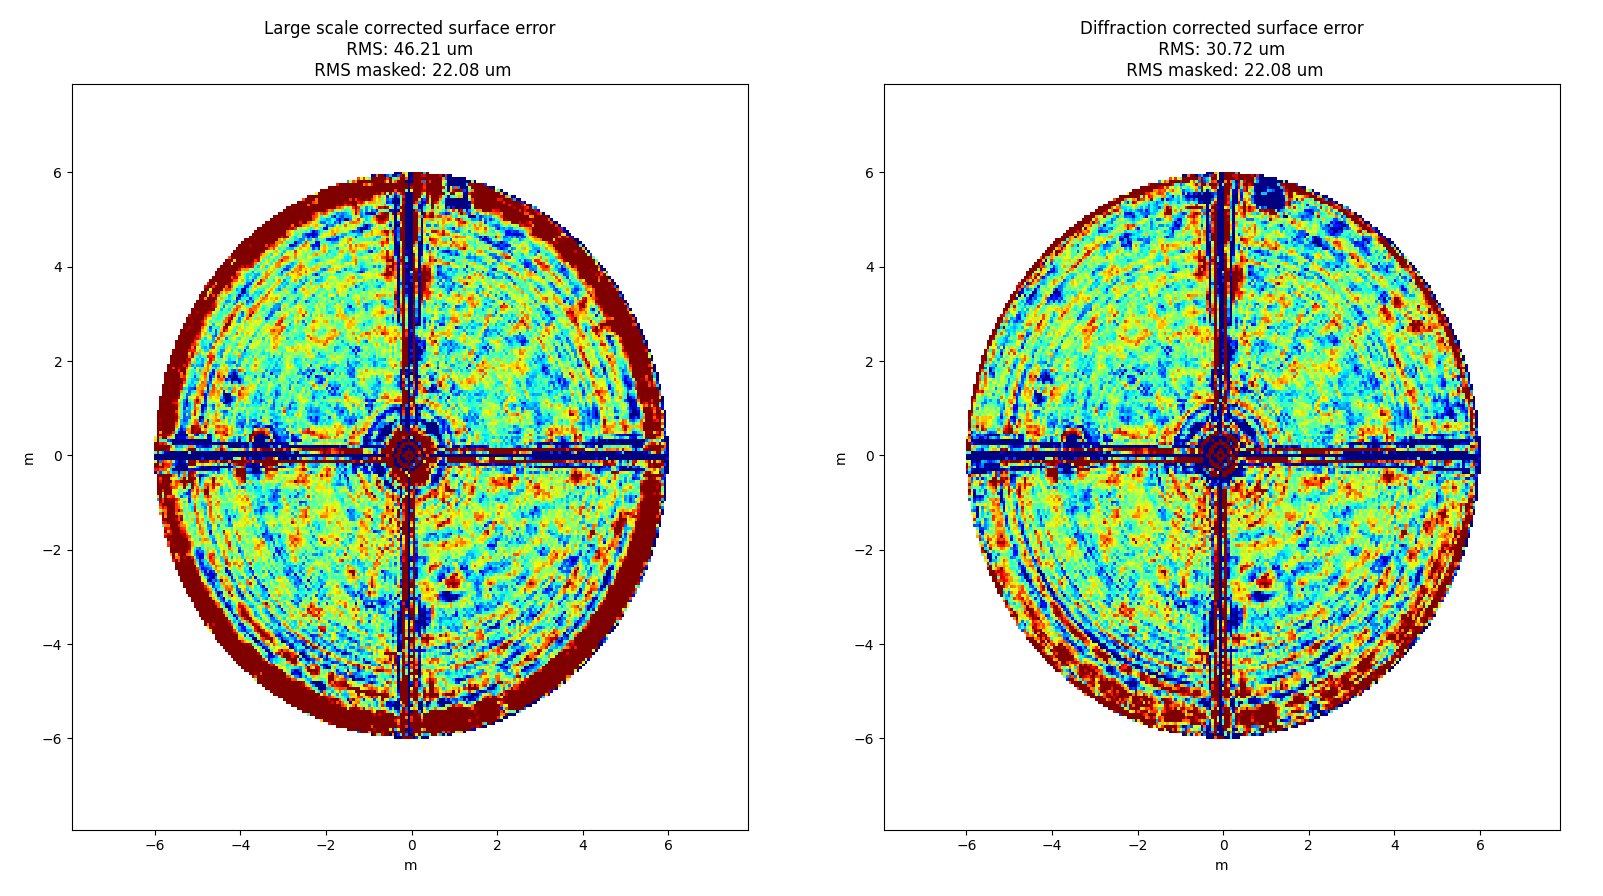
\includegraphics[width=0.9\textwidth]{images/diffraction_correction.png}
    \caption{Example of the effect of the substraction of the diffraction model.}
    \label{fig:diffraction_corrected}
\end{figure}



\subsection{Supporting legs substraction}

